\section*{Úvod}
\addcontentsline{toc}{section}{Úvod}
{\large\sloppy

Hlavním předmětem této práce je vytvoření interpretu pro hru virtuálních robotů. Znamená to tedy vytvořit program, který bude spuštěný na počítači s~veřejným přístupem (s~veřejnou IP adresou) - dále jen \emph{server}, a se kterým budou komunikovat jiné počítačové programy běžící odděleně od \emph{serveru} - dále jen \emph{klienti}.

Tato práce popisuje vytvoření interní architektury aplikace vhodné ke konfigurování a vytváření herních map, správě rozehraných her, klientských herních požadavků na tyto hry a ošetření nestandardních stavů. Je nutno vytvořit konfigurační mechanismus, který by byl schopen na základně parametrů od \emph{klienta} vytvářet nové hry na \emph{serveru} s~různými parametry - jako je výška a šířka mapy, počty herních bloků a další. 

Jako hlavní programovací jazyk byl zvolen programovací jazyk \nameref{subsec:python} především kvůli rychlosti vývoje v~něm, stručnosti a přehlednosti zápisu a také díky jeho výuce na \href{http://www.spseol.cz/}{VOŠ a SPŠE Olomouc}, kde je autor této práce studentem a kde může \emph{server} sloužit pro výuku programování pro pokročilé studenty v~oblasti programování.  

Ve své práci se prvně v~sekci \nameref{sec:theory-analyse} věnuji použité architektuře, objektovým vztahům a administraci s~konfiguračním formulářem. V~sekci \nameref{sec:implementation} jsou probrána implementační rozhodnutí, systém výjimek řídící zpracování herní akce a vnitřní logika konfigurace. Sekce \nameref{sec:used-technologies} vytváří základní přehled o~použitých technologiích přímo podílejících se na běhu aplikace a především jednotkovém testování. Naproti tomu sekce \nameref{sec:used-metatechnologies} popisuje použité technologie, které se nepřímo podíleli na vývoji aplikace, tzv. \emph{metatechnologie}.

}

\section{Teoretický rozbor}
\label{sec:theory-analyse}

\subsection{Rozbor zadání}
\begin{enumerate}
	\item
	{\bfseries Implementujte interpret hry, který bude sloužit pro soutěž virtuálních robotů.}\\
	Z~tohoto bodu plyne zadání vytvořit aplikaci, která bude schopna reprezentovat heru a příjmat jednotlivé klientské herní akce.

	\item
	{\bfseries Interpret postavte tak, aby bylo snadné měnit konkrétní pravidla a styl hry.}\\
	K~aplikaci z~prvního bodu zadání bude nutné přidat konfigurační rozhraní, pomocí které půjdou měnit parametry jednotlivým hrám.

	\item
	{\bfseries Interpret bude umožňovat alespoň tyto styly hry:}
		\begin{enumerate}
			\item Souboj individuálních robotů
			\item Souboj decentralizovaných týmů robotů
			\item Souboj centralizovaných týmů robotů
		\end{enumerate}
	Buď samotným interpretem nebo pomocí konfigurace bude možné přepínat jednotlivé módy hry mezi souboji \emph{jeden bot - jeden bot}, \emph{více botů proti více botům} nebo možnost ovládat z~klientského zařízení více botů.

	\item
	{\bfseries Ve spolupráci s~vedoucím práce zorganizujte jeden ročník této soutěže.}
	Bude potřebné sestavit tutoriál a dokumentaci komunikačního rozhraní serveru pro naprogramování klientských aplikací a následně porovnat různé algoritmické implementace klientů v~různých programovacích jazycích.
\end{enumerate}
\subsection{Návrh architektury aplikace}

\subsubsection{Návrh interní struktury}

\textit{
	V~této sekci se budu zabývat pouze teoretickým návrhem jednotlivých datových a řídící struktur. Popisu použitých algoritmů a jednotlivých implementačních rozhodnutí se budu věnovat v~sekci\fullref{sec:implementation}.
}

O~interní reprezentaci jedné instance hry se stará třída \ic|Game|, která je zodpovědná za striktní přístup klienta do mapy. Zpracovává jednotlivé herní akce klientů, kontroluje jejich validitu a aplikuje změny do mapy. \ic|Game| je sama schopna se vyexportovat do hodnoty, která je následně převeden do formátu \nameref{subsec:json}, jenž je následně distribuován ke klientovi. Při herních akcích překládá výjimky vyvolané interně uloženou mapou na ty zvenku známé. V~případě módu hry s~tahy hlídá \ic|Game| pořadí jednotlivých botů.

Třída \ic|Game| interně využívá třídu \ic|Map| k~uchování stavu hry. Třída \ic|Map| je v~podstatě pouze zapouzdřený kontejner reprezentující vlastní mapu. Je zodpovědná za validní přístup - ošetřuje stavy pro nevalidní přístup mimo rozsah mapy.

Společným předkem pro všechny entity uložené v~mapě je třída \ic|Field|. Jejím nejprimitivnějším potomkem je prázdné pole \ic|EmptyField|.

\begin{sloppypar}
	Existenci bota v~mapě reprezentuje třída \ic|BotField|, která je zopovědná za udržení jeho prostorové orientace a umí se na místě otáčet. V~případě, že se jedná o~hru s~bateriemi, je tato třída nahrazena třídou \ic|LaserBatteryBotField|, která se kromě orientace stará i o~stav baterie. Ten je řízen pomocí metod \ic|LaserBatteryBotField.charge()| pro nabíjení, resp. \ic|drain()| pro vybíjení. Výjimka \ic|CriticalBatteryLevel| je vyvolána v~případě, kdy by mělo dojít k~vybití baterie na kritickou úroveň.
\end{sloppypar}

Mezi další pomomky třídy \ic|Field| patří \ic|BlockField| reprezentující v~mapě pole pevného bloku a \ic|TreasureField| zastupující poklad ve hře.

Třída, která kontroluje jednotlivé instance \ic|Game| v~aplikaci se příznačně nazývá \ic|GameController|. Je zodpovědná delegování klientského herné akce na odpovídající instanci hry. Zároveň zodpovídá za vytváření her, resp. na svém vstupu příjmá instanci potomka třídy \ic|BaseConfiguration|, kterou následně předá do singletonu\footnote{Singleton je návrhový vzor zajišťující právě jednu instanci třídy v~aplikaci.} třídy \ic|MapFactory|, který sestaví instanci mapy.

\ic|MapFactory| je třída zodpovědná za vygenerování mapy v~závislosti na předané konfiguraci. Plný výčet parametů konfigurace lze najít v~tabulce\fullref{table:conf-parameters}.

\begin{table}[H]
	\caption{Seznam možných parametrů herní konfigurace s~parametry}
	\label{table:conf-parameters}
	\centering
	\vspace*{-5pt}
	\begin{tabular}{ l | l | l | l }
		český název & název parametru & vysvětlení & datový typ \\
		\hline
		šířka mapy & \ic|map_width| & počet bloků na šířku mapy & \ic|int| \\
		výška mapy & \ic|map_heigth| & počet bloků na výšku mapy & \ic|int| \\
		počet botů & \ic|bots| & maximální počet botů ve hře & \ic|int| \\
		počet bloků & \ic|blocks| & maximální počet bloků ve hře & \ic|int| \\
		počet pokladů & \ic|treasures| & počet pokladů ve hře & \ic|int| \\
		hra s~tahy & \ic|rounded_game| & hra botů v~pořadí & \ic|bool| \\
		hra s~bateriemi & \ic|battery_game| & hra botů s~bateriemi & \ic|bool| \\
		hra s~lasery & \ic|laser_game| & hra botů s~možností laseru & \ic|bool| \\
	\end{tabular}
	\vspace*{-15pt}
\end{table}

{\titlespacing*{\subsubsection}{0pt}{0.5ex}{0.5ex}
\subsubsection{Návrh vnějšího rozhraní}}

Pro jednotlivé části aplikace je nutné mít různé URL adresy, aby je šlo jednoduše rozlišovat. Přehled URL adres a jejích určení lze najít v tabulce\fullref{table:urls}. Čarou jsou vizuálně odděleny URL adresy patřící hernímu rozhraní a URL adresy určené pro administraci. Také je v tabulce zaznemanána metoda používaná k přístupu na URL.
{
\captionsetup{belowskip=-5pt,aboveskip=0pt}
\begin{table}[H]
	\caption{Seznam URL adres aplikace}
	\label{table:urls}
	\centering
	\begin{tabular}{ B | B | p{37.5ex} }
		URL & metoda & popis \\
		\hline
		/init & GET & vytváří hru a vrací \ic|bot_id| v JSON \\
		/game/<int:bot_id> & GET & vrací hru dle \ic|bot_id| v JSON \\
		/action & POST & příjmá herní akce klientů \\
		/reset & POST & kompletně resetuje aplikaci \\
		/info & GET & vrací JSON výčet enumerací v aplikaci \\
		\hline
		/admin & GET & zobrazuje administraci \\
		/admin & POST & příjmá odeslání konf. formuláře \\
		/admin/<int:bot_id> & GET & vrací admin. detail hry dle \ic|bot_id| \\
		/admin/<int:bot_id> & POST & maže hru dle \ic|bot_id| \\
	\end{tabular}
\end{table}
}

\subsection{Administrace}

\begin{wraptable}[14]{r}{.3\textwidth}
	\caption{Přehled barev v~detailu hry v~administraci}
	\label{table:game-detail-colors}
	\newcommand{\colpic}[1]{\tikz \draw[#1,fill=#1,draw](0,0)circle(7.5pt);}
	\newcolumntype{M}{>{\collectcell{\colpic}}l<{\endcollectcell}}
	\vspace{-10pt}
	\begin{flushright}
		\begin{tabular}{ r | M }
			prázdné pole & emptyfield \\
			poklad & treasurefield \\
			základní bot & botfield \\
			pevný blok & blockfield \\
			rozšířený bot & laserbatterybotfield \\
		\end{tabular}
	\end{flushright}
\end{wraptable}

Pro nastavování aktuálních konfiguračních parametrů z~tabulky\fullref{table:conf-parameters} do akutálně běžící aplikace jsem vytvořil jednoduchou administraci s~formulářem a seznamem rozehraných her. Formulář obsahuje vstupní pole pro všechny parametry s~odpovídajícím typem a pomocí něj je možné změnit parametry nově vytvářených her - jeho detail je možné vidět v~obrázku\fullref{fig:admin-conf-form}. Druhou komponentou v~administraci je seznam příhlášených botů s~možností zobrazení detailu hry a mapy - náhled seznamu možno zhlédnout v~obrázku\fullref{fig:admin-games-list}. V~samotném seznamu lze \textbf{mazat hry}, co jsou \textbf{30 a více sekund neaktivní} - buď samostatně hru po hře nebo hromadně všechny, které odpovídají této podmínce.

\begin{figure}[h]
	\centering
	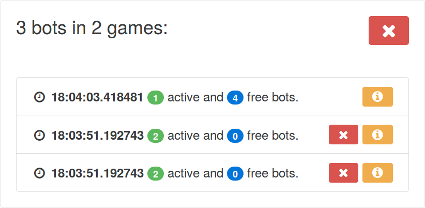
\includegraphics{assets/admin-games-list}
	\caption{Náhled seznamu her v~administraci}
	\label{fig:admin-games-list}
\end{figure}

Při zobrazení detailu je možno vidět celou strukturu mapy, barevně jsou dle tabulky\fullref{table:game-detail-colors} vyznačena jednotlivá herní pole v~\textbf{mapě}, která je s~\textbf{intervalem 2 sekund obnovována}. Náhled tohoto detailu je možno zhédnout v~obrázku\fullref{fig:admin-game-detail}.


\begin{figure}[h]
	\centering
	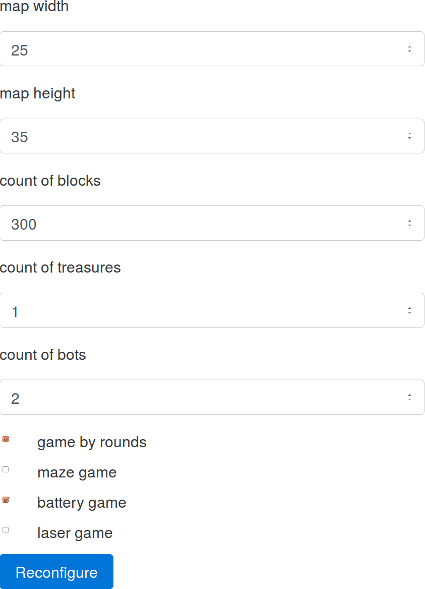
\includegraphics{assets/admin-conf-form}
	\caption{Náhled administračního formuláře pro konfiguraci}
	\label{fig:admin-conf-form}
\end{figure}

\begin{landscape}
\begin{figure}[h]
	\centering
	
\includegraphics[width=\hsize]{assets/admin-game-detail}
	\caption{Náhled detailu hry v~administraci}
	\label{fig:admin-game-detail}
\end{figure}
\end{landscape}
